\section*{ODF Analysis}

\subsection*{Working with ODFs}

\begin{frame}
  \frametitle{Analyzing and Visualizing ODFs in \MTEX}

  \begin{center}
    \begin{tikzpicture}[scale = 0.65,transform shape]
  \definecolor{myblue}{HTML}{92dcec}
  \tikzstyle{every annotation}=[fill=white, font=\sf]
  \tikzstyle{root concept}+=[text width=4.5cm]

  \path[mindmap, concept color=orange!80!]
  node[concept] {\huge \bf ODF\\ Visualization}
  child[grow = 120, concept color=orange!50]
  { node(ebsd) [concept](ebsd2) {\Large ODF Sections}}
  child[grow = 160, concept color=orange!50]
  { node[concept](pf) {\Large Pole Figure}}
  child[grow = -160, concept color=orange!50]
  { node[concept](pf) {\Large Inverse Pole Figure}}
  child[grow = -120, concept color=orange!50]
  { node[concept](pf) {\Large Spectral Plot}};

  \path[mindmap, concept color=blue!50!]
  node[concept] at (5,0){\huge \bf ODF \\Calculations}
  child[grow=75, concept color=blue!30]
  { node(ebsd) [concept](ebsd2) {\Large Volume Portion}}
  child[grow=45, concept color=blue!30]
  { node[concept](pf) {\Large Modal\-Orientation}}
  child[grow=15, concept color=blue!30]
  { node[concept](pf) {\Large Mean\-Orientation}}
  child[grow=-15, concept color=blue!30]
  { node[concept](pf) {\Large Entropy}}
  child[grow=-45, concept color=blue!30]
  { node[concept](pf) {\Large Texture Index}}
  child[grow=-75, concept color=blue!30]
  { node[concept](pf) {\Large Fourier Coefficients}};
\end{tikzpicture}
\end{center}

\end{frame}

\subsection*{Working with ODFs}

\begin{frame}[fragile]
  \frametitle{Texture Characteristics}

Comparing {\bf arbitrary} ODFs
\begin{lstlisting}
calcerror(odf1,odf2,'L1')
\end{lstlisting}

\pause

Volume portions:
\begin{lstlisting}
volume(odf,center,radius)   % the volume of a ball
fibrevolume(odf,h,r,radius) % the volume of a fibre
\end{lstlisting}

\pause

Preferred orientations:
\begin{lstlisting}
o = modalorientation(odf) % the modal orientation
o = mean(odf)             % the mean orientation
\end{lstlisting}

\pause

The shape of the ODF:
\begin{lstlisting}
textureindex(odf)         % the texture index
entropy(odf)              % the entropy
fourier(odf,order)        % the C-coefficients
\end{lstlisting}


\end{frame}


\subsection*{Plotting (Inverse) Pole Figures}

\begin{frame}[fragile]
  \frametitle{Plotting (Inverse) Pole Figures in \MTEX}

  General syntax:
\begin{lstlisting}
plotpdf(odf,Miller(0,1,0),<options>)
plotipdf(odf,[xvector,zvector],<options>)
\end{lstlisting}

Options:
\begin{lstlisting}
antipodal % add antipodal symmetry
complete  % plot complete sphere
\end{lstlisting}


\onslide<1->
\center{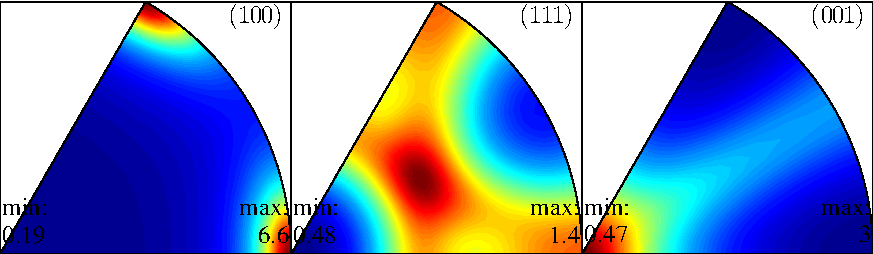
\includegraphics[height=3cm]{pic/ipdf}}

\end{frame}


\subsection*{Plotting an ODF}

\begin{frame}[fragile]
  \frametitle{Plotting  an ODF in \MTEX}

  \begin{columns}
    \begin{column}{6.5cm}
      General syntax:
\begin{lstlisting}
plot(odf,<options>)
\end{lstlisting}

      Sectioning:
      \lstset{emph={sigma},emphstyle={\color{blue}}}
\begin{lstlisting}
alpha, gamma, phi1, phi2
sigma, fibre
\end{lstlisting}

      Options:
\begin{lstlisting}
sections, center, resolution
\end{lstlisting}

      Example:
    \end{column}
    \begin{column}{5cm}
      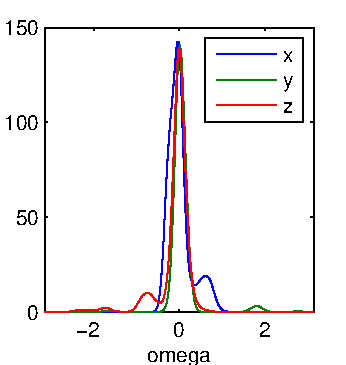
\includegraphics[width=5cm]{pic/radialplot}
    \end{column}
  \end{columns}

\begin{lstlisting}
plot(odf,'fibre',{Miller(0,0,1),zvector},...
  'center',modalorientation(odf))
\end{lstlisting}

%\begin{lstlisting}
%plot(odf,'alpha',[45*degree])
%\end{lstlisting}

\end{frame}


\subsection*{Dubna}

\begin{frame}[fragile]
  \frametitle{A Sigma Plot of the Recalculated Dubna ODF in \MTEX}

\begin{lstlisting}
plot(rec,'sections',18,'FontSize',10)
\end{lstlisting}

\medskip

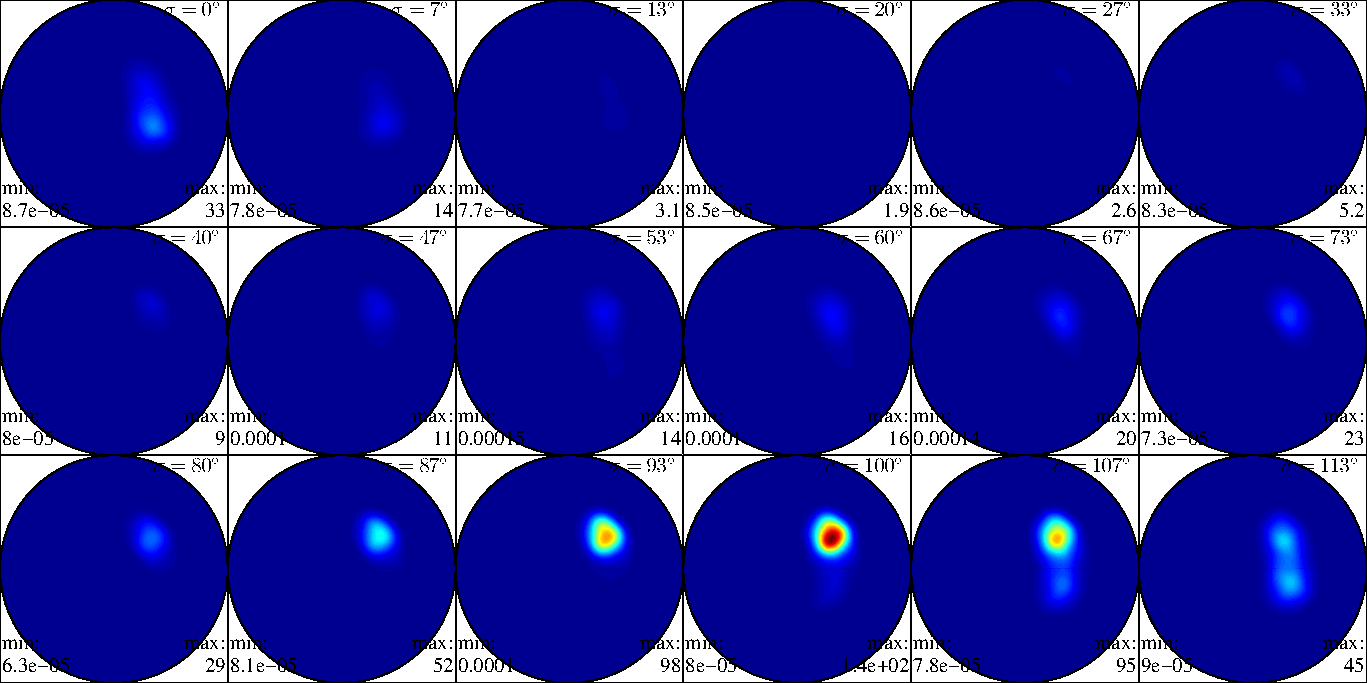
\includegraphics[width=\textwidth]{pic/ODFso9}

\end{frame}

\subsection*{SantaFe}

\begin{frame}[fragile]
  \frametitle{The Classical Plot of the SantaFe ODF in \MTEX}

\begin{lstlisting}
plot(SantaFe,'alpha','sections',18,...
     'projection','plain','gray','contourf')
\end{lstlisting}

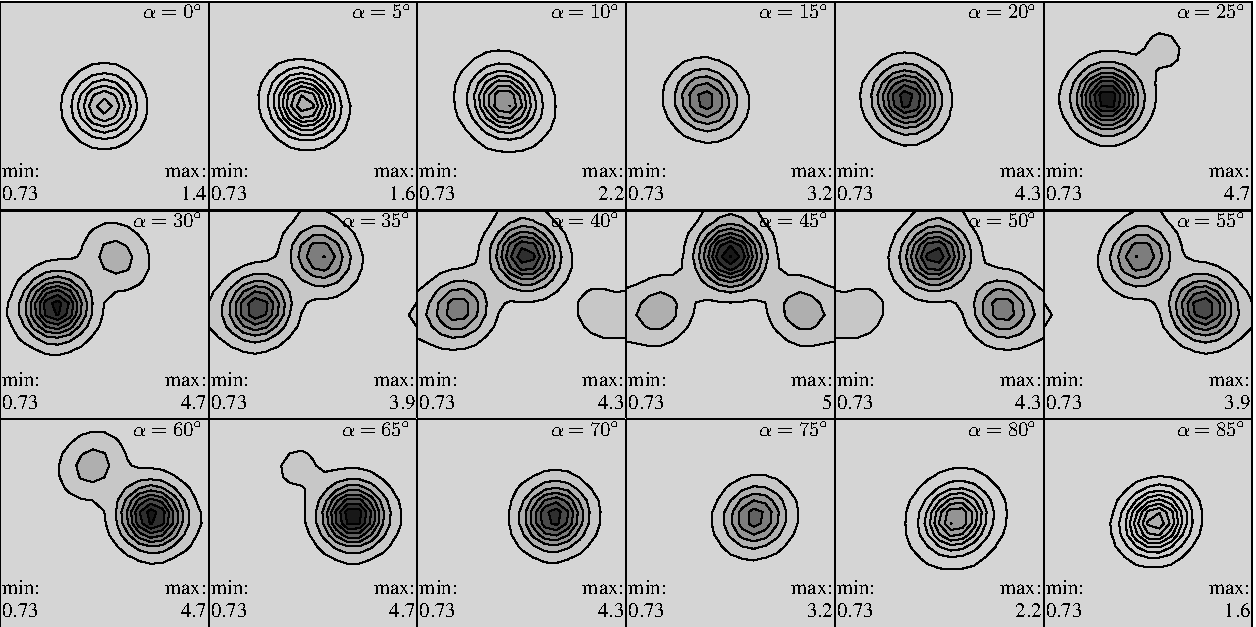
\includegraphics[width=\textwidth]{pic/santafee}

\end{frame}

\subsection*{Exercises}

\begin{frame}

  \begin{Exercise}
    \begin{enumerate}[a)]
      \item Construct a cubic unimodal ODF with mode at $[0 0 1](3 1 0)$.
      \item What is its modal orientation in Euler angles?
      \item Plot some pole figures. Are there pole figures with and without
        antipodal symmetry? What about the inverse pole figures?
      \item Plot the ODF in $\sigma$ and $\phi_{2}$ - sections. How many modes
        do you observe?
      \item Compute the volume of the ODF that is within a distance of 10
        degrees of the mode. Compare the result with the uniform ODF.
    \end{enumerate}
  \end{Exercise}

  \begin{Exercise}
    \begin{enumerate}[a)]
    \item Construct a trigonal ODF that consists of two fibres at
      $h_1 = (0,0,0,1)$, $r_{1} = \mathbf{y}$, $h_2 = (1,0,\bar 1,0)$, $r_{2} = \mathbf{x}$.
    \item Do the two fibres intersect?
    \item What is the modal orientation of the ODF?
    \item Plot the ODF in $\sigma$ and $\phi_{2}$ - sections. How many
      fibres do you observe?
    \item Compute the texture index of the ODF.
    \end{enumerate}
  \end{Exercise}

\end{frame}


%%% Local Variables:
%%% mode: latex
%%% TeX-master: "main"
%%% End:
